\documentclass[../Head/Main.tex]{subfiles}
\begin{document}
\subsection{Model based planner}

The implementation of the model based planner have been designed from a set of key methods namely \texttt{brushfireAlgorithm(int iterations}), \texttt{findCornerPoints()}, \texttt{findCenterPoints()}, \texttt{findLinePoints()}, \texttt{ConnectPoints()}, \texttt{findPathPoints(cv::Point curPos, cv::Point goal)}, \texttt{find(int V)}, \texttt{unionSets(int V1, int V2)} and \texttt{DFS(cv::Point start, cv::Point goal)} from a class called \texttt{brushfire} 

The method \texttt{brusfireAlgorithm(i)} takes and input as the number of iterations one wants to process. After doing so it is possible to get the pixels furthest away from an obstacle and thereby the center points of rooms and doors.   

\begin{figure}[H]
  \begin{subfigure}[b]{0.49\textwidth}
    \centering
    \includegraphics[width=0.9\textwidth]{Roadmaps/brushfire1}
    \caption{Illustration of brushfire in use with 1 iteration}
    \label{fig:Brushfire1}
  \end{subfigure}
  \hfill
   \begin{subfigure}[b]{0.49\textwidth}
    \centering
    \includegraphics[width=0.9\textwidth]{Roadmaps/brushfire}
    \caption{Illustration of brushfire in use with 13 iteration}
    \label{fig:Brusfire2}
  \end{subfigure}
  \end{figure}
  
As seen in figure \ref{fig:Brushfire1} and figure \ref{fig:Brusfire2} the algorithm start by consuming all free pixels closest to the obstacle and iterate through the map. For visualization the pixels furthest away from the obstacle, which have been assigned a value, are pictured green and the once closest to an obstacle are red. This gives a map with connections between rooms. 
  
Now it is possible to find corner and center points via the newly created brushfire map. For this accomplish this two methods were used namely \texttt{findCornerPoints()} and \texttt{findCenterPoints()}.The idea is to compare $pixel(i,j)$ to its neighbours. For instance if $pixel(i-1,j)$ equals $pixel(i+1,j)$ and the center point between them, $pixel(i,j)$, has a different value, it is considered to be a point on a line. The same thing goes for the horizontal case. To find corner points, the $pixel(i-1,j)$ must equal to $pixel(i,j+1)$ and $pixel(i-1,j+1)$ must be different from $pixel(i,j)$. This is just one of the instances of find corner points but the principles is the same for the four cases.           

After completing this operation on the brushfire map it is possible to see corners and center lines in rooms as well as doors. This i visualized in figure \ref{fig:CornersAndCentersOfRoom}.
  
  \begin{figure}[H]
   \begin{subfigure}[b]{0.49\textwidth}
    \centering
    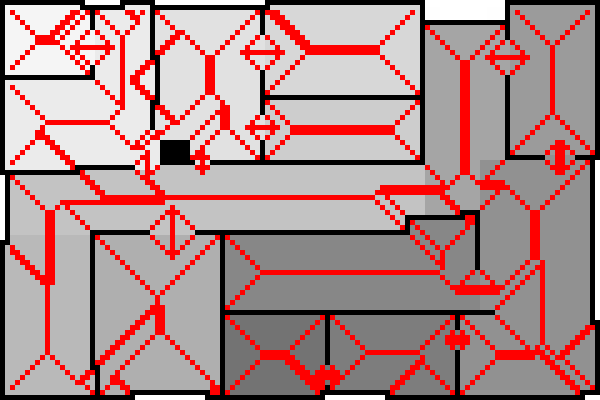
\includegraphics[width=0.9\textwidth]{Roadmaps/RoadPoints1}
    \caption{Illustration of findCornerPoints and centerPoints in use}
    \label{fig:CornersAndCentersOfRoom}
  \end{subfigure}
  \hfill
   \begin{subfigure}[b]{0.49\textwidth}
    \centering
    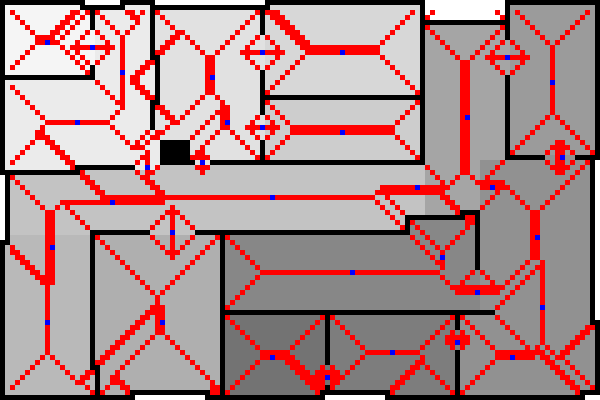
\includegraphics[width=0.9\textwidth]{Roadmaps/RoadPoints}
    \caption{Illustration of findLinePoints in use}
    \label{fig:LinePoints}
  \end{subfigure}
  \end{figure}

It is quite interesting to see the amount of possible points that can be used to make connections between rooms after using the method just mentioned. Because the goal is to make full connections between all rooms, the vertical and horizontal lines on figure\ref{fig:CornersAndCentersOfRoom} is going to be taken into consideration as it will satisfy the objective of finding a path between all points without hitting an obstacle. The method \texttt{findLinePoints()} was created to solve this task. The method iterates through a matrix containing all values on the map and pushes the found line points on a vector and then saves the center point on that detected line. It is worth noting that there are horizontal as well as vertical lines. This will lead to a set of lines points as shown in figure \ref{fig:LinePoints}. 

Now in the creation of the road map every point is considered to be a vertex and a connection between two vertexes is an edge. Now the interesting part is to find out which vertexes that can be connected to one another without hitting an obstacle. Because all obstacles have been assigned the value of 1 it is possible to iterate through the map and see if $pixel(i,j) == 1$ is located somewhere on the edge between these two vertexes. If that is not the case, the edge is considered valid and saved as an edge and thereby a possible connection between two vertexes. This is done in the method \texttt{connectPoints()}. It is critical to point out that Kruskal's algorithm is used in this method as it is a big part of the procedure of connecting the vertexes by the shortest edge first (Kruskal's algorithm was discussed in the design phase of the model based planner). 

  \begin{figure}[H]
   \begin{subfigure}[b]{0.49\textwidth}
    \centering
    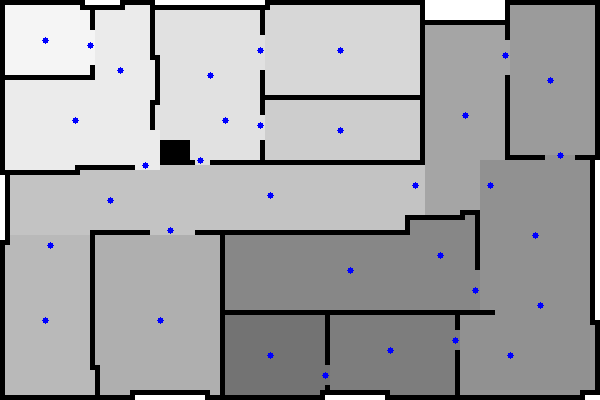
\includegraphics[width=0.9\textwidth]{Roadmaps/RoadMap1}
    \caption{Illustration of the vertexes on the map}
    \label{fig:Vertexes}
  \end{subfigure}
  \hfill
   \begin{subfigure}[b]{0.49\textwidth}
    \centering
    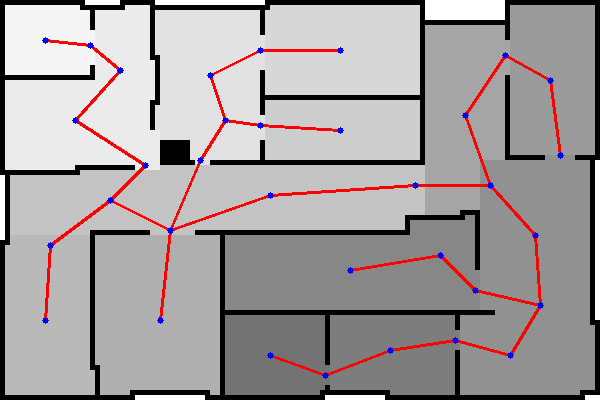
\includegraphics[width=0.9\textwidth]{Roadmaps/RoadMap}
    \caption{Illustration of the connected map between vertexes via edges}
    \label{fig:VertexesAndEdges}
  \end{subfigure}
  \end{figure}  
  
One can see all the vertexes in figure \ref{fig:Vertexes} and there connections to one another after using the method \texttt{connectPoints()} in figure \ref{fig:VertexesAndEdges}. Notice that the edges between vertexes do not contain any cycles which is one of the big advantages of using Kruskal's algorithm and thereby making it easier to make a path between vertexes.  

Now the method \texttt{findPathPoints(c,p)} can be used to generate a map from an initial position to a target location giving the two points as parameters. \texttt{FindPathPoints} uses the methods \texttt{find(int V)}, \texttt{unionSets(V1,V2)} and \texttt{DFS(s,g)} which are already discussed in the design phase. The outcome of this method is a set of points starting from an initial position to a target location.        

  \begin{figure}[H]
   \begin{subfigure}[b]{0.49\textwidth}
    \centering
    \includegraphics[width=0.9\textwidth]{KruskalsAndDFSTest/Pathtest1}
    \caption{Illustration of a path between 3 edges}
    \label{fig:Vertexes}
  \end{subfigure}
  \hfill
   \begin{subfigure}[b]{0.49\textwidth}
    \centering
    \includegraphics[width=0.9\textwidth]{KruskalsAndDFSTest/Pathtest3}
    \caption{Illustration of a path between 16 edges}
    \label{fig:VertexesAndEdges}
  \end{subfigure}
  \end{figure}  

Several test were made to see how well the model based planner worked. First of all 14 test was conducted to see if the robot was able to find all the rooms in the bigworld map starting from the origin of the map. The average success rate of this test was 100\% meaning that it found a way to all 14 rooms. The test also showed that the average distance to obstacle was 2.345 meters. Another important factor was that it was able to run through the entire map starting from the origin and then to all rooms from room 1 to 14 which can be seen in figure \ref{fig:brushfireCompletePath}. 

  \begin{figure}[H]
   \begin{subfigure}[b]{0.49\textwidth}
    \centering
    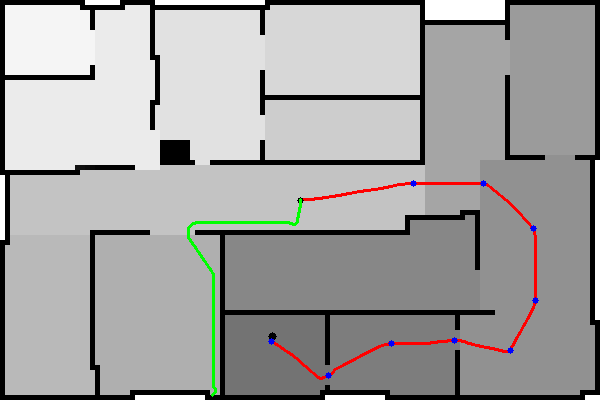
\includegraphics[width=0.9\textwidth]{Modelbased_vs_Sensorbased/brushfireAndBugTest14}
    \caption{Illustration of findCornerPoints and centerPoints in use}
    \label{fig:brushfireToRoom14}
  \end{subfigure}
  \hfill
   \begin{subfigure}[b]{0.49\textwidth}
    \centering
    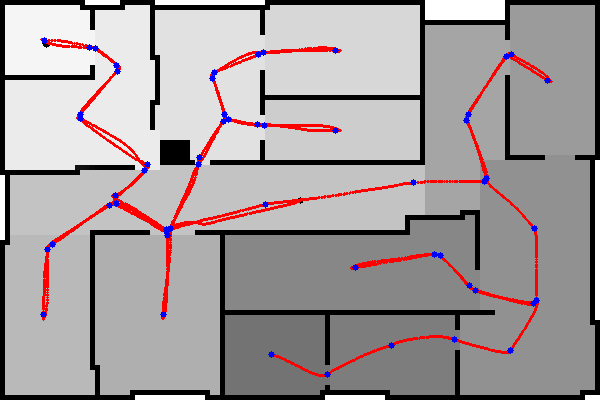
\includegraphics[width=0.9\textwidth]{Modelbased/brushfireTest15}
    \caption{Illustration of findLinePoints in use}
    \label{fig:brushfireCompletePath}
  \end{subfigure}
  \end{figure}  

Figure \ref{fig:brushfireToRoom14} shows the working of the brushfire algorithm going from the origin to room 14 marked with a red path. The green path is the test of the sensor based planer. One can see that the model based planer follows the graph nicely and ends up in the target location. Another test using the model based planner was performed to test the fuzzy control and see if the robot was able to collect marbles. The was concluded that the fuzzy control works and that the robot was able to find marbles where on of the test resulted in a full search of all rooms with 10 marbles collected as seen in figure \ref{fig:brushfireCompletePath}. But unfortunately gazebo crashed several times while collecting marbles which affected the results.
  \begin{figure}[H]
   \begin{subfigure}[b]{0.49\textwidth}
    \centering
    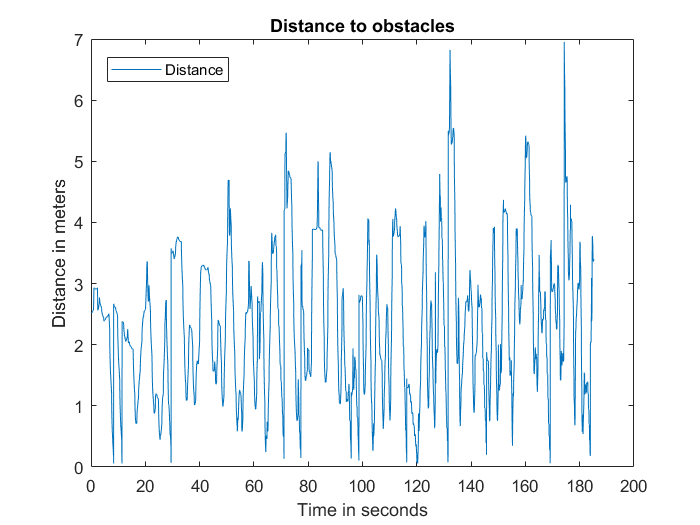
\includegraphics[width=0.9\textwidth]{MatlabPlots/MarblesTest4}
    \caption{Illustration of findCornerPoints and centerPoints in use}
    \label{fig:matlabPlotMarbletest14}
  \end{subfigure}
  \hfill
   \begin{subfigure}[b]{0.49\textwidth}
    \centering
    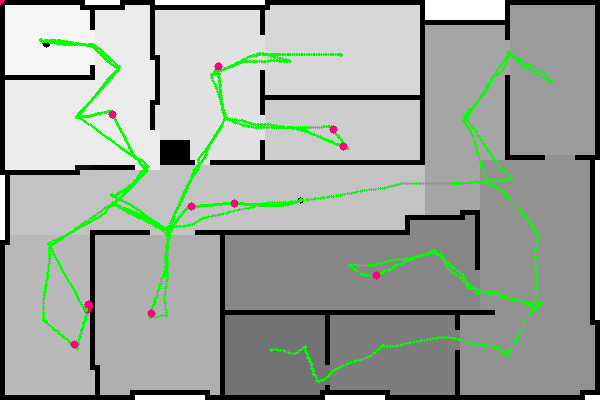
\includegraphics[width=0.9\textwidth]{Modelbased/brushfireMarble4}
    \caption{Illustration of findLinePoints in use}
    \label{fig:brushfireMarbleFindingTest}
  \end{subfigure}
  \end{figure}  

In figure \ref{fig:matlabPlotMarbletest14} one can see when a marble is collected when the spike of a distance to an obstacle is very close to zero. More test results can be seen in section \ref{subsec:testCollectMarbles}.

\end{document}